\documentclass[12pt,fleqn]{article}\usepackage{../common}
\begin{document}
Algilayicilardan Gelen Gauss Dagilimlarinin Fuzyonu (Gaussian Sensor Fusion)

Diyelim ki tek boyutlu ortamda bir buyuklugu mesela bir lokasyon bilgisi
$x$'i, iki kere olcuyoruz, ve bu olcumu iki degisik algilayiciya
yaptiriyoruz. Yani iki alet bir cismin oldugu yeri bize geri donduruyor, bu
bilgilerde belli olcude gurultu var ki bu belirsizlik aletler yuzunden
olabilir. Diyelim ki iki $z_1,z_2$ olcumu icin iki degisik belirsizlik
(uncertainty) $\sigma_1,\sigma_2$. 

Soru su, bu iki olcumu kullanarak daha iyi bir $x$ tahmini yapabilir miyiz?

Bunun iki olcumu bir sekilde birlestirmemiz gerekiyor. Her olcumu Gaussian
/ Normal dagilim olarak modelleyebiliriz, o zaman iki Normal dagilimi bir
sekilde birlestirmemiz (fusion) lazim. Olcumleri temsil etmek icin Gaussian
bicilmis kaftan. Olcumdeki belirsizligi standart sapma (standart deviation)
uzerinden rahatlikla temsil edebiliriz. Peki birlestirimi nasil yapalim? 

Bu tur problemlerde maksimum olurluk (maximum likelihood) kullanilmasi
gerektigini asagi yukari tahmin edebiliriz, cunku maksimum olurluk verinin
olurlugunu maksimize ederek bilinmeyen parametreleri tahmin etmeye
ugrasir. Cogunlukla bu teknigi hep {\em tek} bir dagilim baglaminda
gormusuzdur herhalde (ders kitaplarinda vs), o tek dagilima degisik veri
noktalari verilerek olasilik sonuclari carpilir, ve bu maksimize edilmeye
ugrasilir. Fakat maksimum olurluk illa tek bir dagilimla kullanilabilir
diye bir kural yok. Ustteki problemde iki olcumu iki Gaussian ile temsil
ederiz (buna mecburuz, iki degisik belirsizlik var), ve bu iki Gaussian'a
verilen iki olcum noktasini olurlugunu bu Gaussian'larin sonuclarini
carparak elde edebiliriz. Peki bilinmeyen $x$ nedir? Onu da Gaussian'in
orta noktasi (mean) olarak aliriz! Yani

$$ L(x) = p(z_1|x,\sigma_1) p(z_2|x,\sigma_2) $$

$$ L(x) \sim \exp{\frac{-(z_1-x)^2}{2\sigma_1^2} } 
\times \exp \frac{-(z_2-x)^2}{2\sigma_2^2} $$

1D Gaussian formulunu hatirlarsak, 

$$ p(z;x,\sigma) = \frac{1}{\sigma\sqrt{2\pi}} 
\exp \bigg\{ - \frac{(z-x)^2}{2\sigma^2}  \bigg\}
 $$

Ders notlari [1]'de iki ustteki formulun nasil maksimize edilerek bir
$x_{MLE}$ formulune erisildigini gorebiliriz. Ustteki formul basindaki
sabit kisminin $L(x)$ formulunde kullanilmadigini goruyoruz, cunku
maksimizasyon acisindan dusunursek, o kisim tekrar tekrar carpilacak ve,
hesaplamaya calistigimiz degiskenler acisindan en azindan bu ek buyukluk
bir fark yaratmayacakti.

Ustteki metot ta isler. Fakat biz alternatif olarak daha degisik (temiz?)
bir yoldan gidecegiz. Elimizdeki her iki olcumu iki farkli 1 boyutlu
Gaussian olarak temsil etmek bir yontemdir. Diger bir yontem su
olabilir. \textbf{2 boyutlu} bir Gaussian yaratiriz, ve iki olcumu tek bir
2 boyutlu vektor icinde belirtiriz, ve tek bir olasilik hesabi $p(z;x,\Sigma)$ 
yapariz. Belirsizlikler ne olacak? Olcum belirsizliklerini bu 2D
Gaussian'in kovaryansinda capraza (diagonal) koyariz, capraz disindaki
matris ogeleri sifir olursa boylece iki olcumun birbirinden bagimsizligini
temsil etmis oluruz. Maksimizasyon nasil olacak? Tek bir olcumun
olasiligini maksimize etmek mumkun, cunku bu hesap sirasinda bilinmeyen
degiskenleri iceren yeni bir formul ortaya cikacak. 

Cok boyutlu Gaussian'i hatirlayalim (artik $z,x$ birer vektor),

$$ p(z;x,\Sigma) = 
\frac{ 1}{(2\pi)^{k/2} \det(\Sigma)^{1/2}} \exp 
\bigg\{ 
-\frac{ 1}{2}(z-x)^T\Sigma^{-1}(z-x)
\bigg\} $$

Kisaca,

$$ =  \frac{ 1}{C} \exp 
\bigg\{ 
-\frac{ 1}{2}(z-x)^T\Sigma^{-1}(z-x)
\bigg\} $$

Bir numara, $\exp$ ve parantez ici negatif ibareden kurtulmak icin
$-\ln p$ alalim,

$$ -\ln p(z) = 
\frac{ 1}{2}(z-x)^T\Sigma^{-1}(z-x)
$$

Simdi iki olcumu, belirsizligi vektor / matris ogeleri olarak gosterelim, 

$$ = \frac{1}{2}  
\left[\begin{array}{c}
z_1-x \\ z_2-x
\end{array}\right]^T
\left[\begin{array}{cc}
\sigma_1^2 & 0 \\
0 & \sigma_2^2 
\end{array}\right]^{-1}
\left[\begin{array}{c}
z_1-x \\ z_2-x
\end{array}\right]
$$

Capraz matrisin tersini almak icin caprazdaki ogelerin tersini almak
yeterlidir,

$$ = \frac{1}{2}  
\left[\begin{array}{c}
z_1-x \\ z_2-x
\end{array}\right]^T
\left[\begin{array}{cc}
\sigma_1^{-2} & 0 \\
0 & \sigma_2^{-2} 
\end{array}\right]
\left[\begin{array}{c}
z_1-x \\ z_2-x
\end{array}\right]
$$

$$ = \frac{1}{2}  
\left[\begin{array}{cc}
\sigma_1^{-2}(z_1-x) & \sigma_2^{-2} (z_2-x)
\end{array}\right]
\left[\begin{array}{c}
z_1-x \\ z_2-x
\end{array}\right]
$$

$$ = 
\frac{1}{2}\sigma_1^{-2}(z_1-x)^2 + \frac{1}{2}\sigma_2^{-2} (z_2-x)^2
$$

Maksimize etmek icin bilinmeyen $x$ degiskenine gore turev alip sifira
esitleyebiliriz, 

$$ 
\sigma_1^{-2}z_1-\sigma_1^{-2}x + \sigma_2^{-2}z_2-\sigma_2^{-2}x = 0
$$

$x$ uzerinden gruplarsak,

$$ 
-x(\sigma_1^{-2}+\sigma_2^{-2}) + \sigma_1^{-2}z_1+ \sigma_2^{-2}z_2 = 0
$$

Gruplanan kismi esitligin sagina alalim,

$$ 
\sigma_1^{-2}z_1+ \sigma_2^{-2}z_2 = x(\sigma_1^{-2}+\sigma_2^{-2}) 
$$

$$ 
\frac{\sigma_1^{-2}z_1+ \sigma_2^{-2}z_2 }{\sigma_1^{-2}+\sigma_2^{-2}}= x_{MLE}
$$

Ornek

Elimizde belirsizlikleri $\sigma_1=10,\sigma_2=20$ olan iki algilayici
var. Bu algilayicilar ayni obje hakkinda $z_1=130,z_2=170$ olarak iki olcum
gonderiyorlar. Bu olcumleri birlestirelim. Hatirlarsak $10^{-2}$ ile
carpmak $10^{2}$ ile bolmek ayni sey.

$$ x_{MLE} =
\frac{130/10^2 + 170/20^2}{1/10^2 + 1/20^2} = 138.0
$$

Sonucun belirsizligi daha az olan olcume daha yakin ciktigini goruyoruz. 

Cok Boyutlu Gaussian Fuzyon

Peki ya elimizdeki birden fazla olan olcumlerin herbiri cok boyutlu ise? 

O zaman yine maksimum olurluk uzerinden bir formul turetebiliriz. Bu
durumda iki ayri dagilim olacaktir,

$$ p(z_1;x,\Sigma_1) =  \frac{ 1}{C_1} \exp 
\bigg\{ 
-\frac{ 1}{2}(z_1-x)^T\Sigma_1^{-1}(z_1-x)
\bigg\} $$

$$ p(z_2;x,\Sigma_2) =  \frac{ 1}{C_2} \exp 
\bigg\{ 
-\frac{ 1}{2}(z_2-x)^T\Sigma_2^{-1}(z_2-x)
\bigg\} $$

Orta nokta $x$ her iki formulde ayni cunku degismeyen olan o; ayni orta
nokta icin tahmin uretmeye ugrasiyoruz.  Simdi bildik maksimum olurluk
hesaplarina biraz daha yaklastik. Daha once $\ln$ alarak $\exp$'yi
yoketmistik. Bunun bir diger faydasi $\ln$ alininca carpimlarin toplama
donusmesidir, 

$$ L = p(z_1;x,\Sigma_1) p(z_2;x,\Sigma_2) 
$$

$$ -\ln L = -\ln p(z_1;x,\Sigma_1) -\ln p(z_2;x,\Sigma_2) 
$$

$$ -\ln L = 
\frac{ 1}{2}(z_1-x)^T\Sigma_1^{-1}(z_1-x) + 
\frac{ 1}{2}(z_2-x)^T\Sigma_2^{-1}(z_2-x)
$$

Simdi esitligin sag tarafinin $x$'e gore turevini alalim, vektor ve matris
baglaminda turev nasil alinir? Herhangi bir $M$'in simetrik oldugu
durumlarda

$$ \frac{\partial}{\partial x}[x^TMx] = 2Mx $$

oldugunu biliyoruz [2]. O zaman turev sonucu soyle olur, 

$$ 
(z_1-x)^T\Sigma_1^{-1} +  (z_2-x)^T\Sigma_2^{-1}
$$

Sifira esitleyip cozelim, 

$$ 
(z_1-x)\Sigma_1^{-1} +  (z_2-x)\Sigma_2^{-1} = 0
$$

$$ 
z_1\Sigma_1^{-1} - x\Sigma_1^{-1} + z_2\Sigma_2^{-1} - x\Sigma_2^{-1} = 0
$$

Yine $x$ altinda gruplayalim,

$$ 
-x(\Sigma_1^{-1} + \Sigma_2^{-1}) + z_1\Sigma_1^{-1}  + z_2\Sigma_2^{-1}  = 0
$$

$$ 
z_1\Sigma_1^{-1}  + z_2\Sigma_2^{-1}  = x(\Sigma_1^{-1} + \Sigma_2^{-1}) 
$$

Eger iki belirsizligin toplamini $\Sigma_x^{-1}$ olarak ozetlersek, yani 

$$ 
\Sigma_x^{-1} = \Sigma_1^{-1} + \Sigma_2^{-1}
$$

O zaman ana formule donelim,

$$ 
z_1\Sigma_1^{-1}  + z_2\Sigma_2^{-1}  = x\Sigma_x^{-1}
$$


$$ 
\Sigma_x (z_1\Sigma_1^{-1}  + z_2\Sigma_2^{-1}) = x_{MLE}
$$

Ornek

Elimizde iki tane iki boyutlu olcum var, 

$$ z_1 = \left[\begin{array}{c}
1 \\ 1
\end{array}\right], 
z_2 = \left[\begin{array}{r}
2 \\ -1
\end{array}\right] 
$$

Olcumler iki degisik algilayicidan geliyor, belirsizlikleri

$$ 
\Sigma_1 = 
\left[\begin{array}{cc}
1 & 0 \\ 0 & 4
\end{array}\right], 
\Sigma_2 = 
\left[\begin{array}{cc}
4 & 0 \\ 0 & 1
\end{array}\right]
 $$

Nihai olcum nedir? 

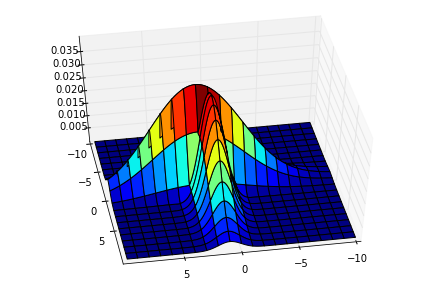
\includegraphics[height=4cm]{fusion_1.png}

Resimde once ilk olcum, sonra onunla yanyana olacak ikinci olcum koyulmus. 

$$ \Sigma_x^{-1} = \Sigma_1^{-1} + \Sigma_2^{-1}  =
\left[\begin{array}{cc}
1 & 0 \\ 0 & 0.25
\end{array}\right] + 
\left[\begin{array}{cc}
0.25 & 0 \\ 0 & 1
\end{array}\right] =
\left[\begin{array}{cc}
1.25 & 0 \\ 0 & 1.25
\end{array}\right] 
$$

Tersini alalim (daha dogrusu tersin tersini almis oluyoruz)

$$ \Sigma_x =
\left[\begin{array}{cc}
0.8 & 0 \\ 0 & 0.8
\end{array}\right] 
$$

$$ x_{MLE} =  \Sigma_x (z_1\Sigma_1^{-1}  + z_2\Sigma_2^{-1}) $$

$$ 
x_{MLE} =
\left[\begin{array}{cc}
0.8 & 0 \\ 0 & 0.8
\end{array}\right] 
\bigg(
\left[\begin{array}{cc}
1 & 0 \\ 0 & 0.25
\end{array}\right] 
\left[\begin{array}{c}
1 \\ 1
\end{array}\right]  + 
\left[\begin{array}{cc}
0.25 & 0 \\ 0 & 1
\end{array}\right] 
\left[\begin{array}{r}
2 \\ -1
\end{array}\right]  
\bigg) = 
\left[\begin{array}{r}
1.2 \\ -0.6
\end{array}\right]  
$$

Sonuc grafiklenirse suna benzer,

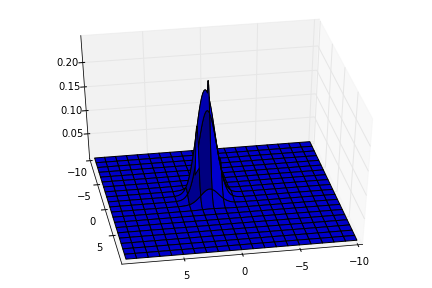
\includegraphics[height=4cm]{fusion_2.png}

[1] \url{www.robots.ox.ac.uk/~az/lectures/est/lect34.pdf}

[2] Hart, Duda, {\em Pattern Classification}

\end{document}
